\section{Versuchsaufbau und Durchführung}

\noindent Um die Wärmeleitfähigkeit unterschieldlicher Materialien zu untersuchen werden mit einem Xplorere GLX als Messgeräte die Temperaturen an den Thermoelementen abgegriffen.

\subsection{Versuchsaufbau}
Auf einer Platte sind Probenstäbe mit unterschiedlichen Querschnittsflächen aus Aluminium, Edelstahl und zwei mal Messing aufgebracht.
Dies ist in Abbildung \ref{img:plat} abgebildet.\\
Diese Stäbe können alle von einem Peltierelement simultan erhitzt werden. Auf den Stäben sollte dabei zu jedem Zeitpunkt die Isolation liegen.\\
An das Peltierelement können für die in den Messreihen benötigten unterschiedlichen Verfahren unterschiedliche Spannungen angelegt werden.
Für die statische Methode entspricht dies einer Spannung von $U_p =\SI{5}{\volt}$ und für die dynamische Methode $U_p =\SI{8}{\volt}$.\\
An den in Abbildung \ref{img:plat} eingezeichneten Thermoelementen lassen sich mit dem in Abbildung \ref{img:log} dargestellten Datenlogger die Temperaturen der Stäbe aufnehmen.
Diese Elemente sind $\increment x = \SI{3}{\centi\metre}$ von einander entfernt.

\begin{figure}[ht]
    \centering
    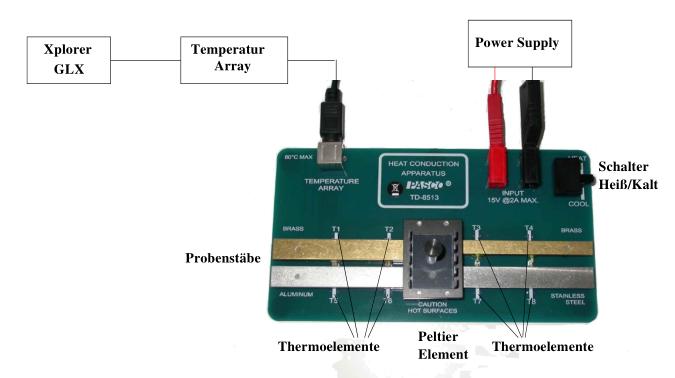
\includegraphics[width=0.7\textwidth]{latex/images/platine.PNG}
    \caption{Die Platte mit dem Peltierelement und denn aufgebrachten Probestäben \protect \cite{V204}}
  \label{img:plat}
\end{figure}

\begin{figure}[ht]
    \centering
    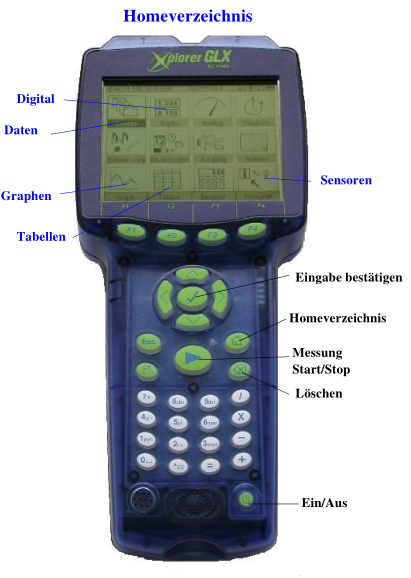
\includegraphics[width=0.4\textwidth]{latex/images/geraet.PNG}
    \caption{Der Datenlogger Xplorer GLX, mit dem die Messwerte aufgenommen werden  \protect \cite{V204}}
  \label{img:log}
\end{figure}

\subsection{Durchführung}

\noindent Nach dem alle auf der Platte aufgetragenen Elemente der Abbildung \ref{img:plat} entsprechend verkabelt wurden, 
können am Datenlogger die für die Messung benötigten Einstellungen getätigt werden.

\subsubsection{Statische Methode}
\noindent
Für die statische Methode entspricht dies dem Einstellen der Abtastrate zu $\increment T= \SI{0.2}{\second}$.
Dabei werden dann bei einer an das Peltierelement angelegten Spannung $U_P=\SI{5}{\volt}$ für $700$ Sekunden die Temperaturen aller Thermoelemente aufgenommen.\\
Hieraus lassen sich dann die Temperaturverläufe der einzelnen Stäbe grafisch darstellen. Zusätzlich lässt sich hieraus der Wärmestrom bestimmen und ablesen welcher Stab die beste Wärmeleitfähigkeit besitzt.\\
Für den Edelstahlstab sollen dann auch noch die Differenzen zwischen den Temperaturen an den Messpunkten grafisch dargestellt werden.

\subsubsection{Dynamische Methode}
\noindent
Wenn die Stäbe hinreichend abgekühlt sind können sie bei $U_P=\SI{8}{\volt}$ wieder erhitzt werden.\\
Dabei ist aber zu beachten, dass für das Angström-Verfahren der Stab periodisch erhitzt werden muss.
Deswegen muss periodisch, manuell zwischen erhitzen und abkühlen hin und her geschaltet werden.\\
Für die erste Messreihe wird eine Welle mit der der Periodendauer $T=\SI{80}{\second}$ erzeugt werden.
Deswegen muss alle $T=\SI{40}{\second}$ umgeschaltet werden. Die Werte sollen dann anch zehn Perioden ausgelesen werden.\\
Hiermit soll dann für den breiten Messingstab der Temperaturverlauf grafisch dargestellt werden. Zusätzlich soll auch noch $\kappa$ berechnet und aus den Grafiken die Phasendifferenz $\increment t$ der Wellen bestimmt werden.\\\\

\noindent
Nach hinreichendem Abkühlen wird diese Messung mit sechs Perioden deren Dauer $T=\SI{200}{\second}$ entspricht, wiederholt.\\
Dabei wird die Auswertung zu der vorigen Messreihe identisch durchgeführt, nur auf den Edelstahlstab bezogen.
